%% Machine Learning with Applications — Elsevier
%% Document class: elsarticle (preprint, single-column for review)
%% Bibliography: APA 7th (natbib + elsarticle-harv style)
%%
%% Compile:
%%   pdflatex main
%%   bibtex   main
%%   pdflatex main
%%   pdflatex main

\documentclass[preprint,12pt,authoryear]{elsarticle}

%% ── Packages ──────────────────────────────────────────────────────────────
\usepackage{amsmath,amssymb,amsfonts}
\usepackage{graphicx}
\usepackage{booktabs}
\usepackage{array}
\usepackage{multirow}
\usepackage[table,xcdraw]{xcolor}
\usepackage{hyperref}
\usepackage{cleveref}
\usepackage{lineno}
\usepackage{microtype}
\usepackage{siunitx}
\usepackage{bm}          % bold math
\usepackage{caption}
\usepackage{subcaption}
\usepackage[utf8]{inputenc}
\usepackage[T1]{fontenc}

%% Line numbers (required for review)
\linenumbers

%% SI units setup
\sisetup{separate-uncertainty=true, group-separator={,}}

%% Hyperref colours
\hypersetup{
    colorlinks=true,
    linkcolor=blue!70!black,
    citecolor=blue!60!black,
    urlcolor=blue!60!black
}

%% ── Macros ────────────────────────────────────────────────────────────────
\newcommand{\CR}[1]{CR_{2,\text{#1}}}          % CR2 variant
\newcommand{\RMSE}{\mathrm{RMSE_{CV}}}
\newcommand{\Rsq}{R^{2}_{\mathrm{CV}}}
\newcommand{\nd}{N_{\mathrm{d}}}               % number of dampers
\newcommand{\np}{n_{\mathrm{s}}}               % number of stories
\newcommand{\etad}{\eta}                        % damper density N_d/n_s
\newcommand{\Mf}{M_{\!f}}                      % friction moment
\newcommand{\ha}{h_a}                          % lever arm
\newcommand{\KM}{\,\si{kN{\cdot}m}}

%% ── Journal front matter ──────────────────────────────────────────────────
\journal{Machine Learning with Applications}

\begin{document}

\begin{frontmatter}

\title{Machine Learning-Based Optimization of Rotational Friction Dampers
       in Multi-Story Steel Moment-Resisting Frames Under Seismic Loading}

\author[uaq]{E.~Ponce}
\author[i2m]{H.~Yañez-Godoy\corref{cor1}}
\cortext[cor1]{Corresponding author.}
\ead{humberto.yanez-godoy@u-bordeaux.fr}

\address[uaq]{Universidad Autónoma de Querétaro, Facultad de Ingeniería,
              Cerro de las Campanas s/n, Querétaro, México}
\address[i2m]{Arts et Metiers Institute of Technology, University of Bordeaux,
              Centre National de la Recherche Scientifique (CNRS),
              Bordeaux INP, I2M, UMR 5295, 33400 Talence, France}

%%─── Abstract ─────────────────────────────────────────────────────────────
\begin{abstract}
This study presents a machine learning surrogate framework for the seismic
optimization of rotational friction dampers (RFDs) in multi-story steel
moment-resisting frames (SMRFs). A Latin Hypercube Sampling (LHS) design
generated 1\,000 structurally diverse shear-frame models spanning 3--20 stories
and fundamental periods $T_1 \in [0.3,\,3.0]$\,s, each evaluated under
approximately 50 RFD configurations and 8 real seismic records, yielding
$\approx$434\,000 nonlinear time-history simulations solved via the
Non-Smooth Dynamics (NSD) method. The composite performance index $CR_2$
--- integrating peak displacement, absolute acceleration, and base shear
normalized with respect to the undamped reference structure --- was
aggregated over records into three statistical scenarios: median (typical),
P10 (favorable), and P90 (conservative). Four regression models were
trained using GroupKFold cross-validation to prevent structural data
leakage. XGBoost achieved the best generalization with cross-validated
$\Rsq$ of 0.92, 0.93, and 0.84 for $\CR{med}$, $\CR{P10}$, and
$\CR{P90}$, respectively. Feature importance analysis reveals that damper
density $\etad = \nd/\np$ is the dominant design driver
($r=-0.73$ with $CR_2$), substantially outweighing the absolute damper
count ($r=-0.45$). Within-structure analysis demonstrates that 80\,\% of
the achievable performance gain is captured at $\etad \approx 0.85$ for
mid-to-high-rise frames (6--20 stories), establishing a
practical diminishing-returns threshold that quantitatively extends the
energy-based findings of \citet{Jarrahi2020sdee}. The ML surrogate enables
near-instantaneous evaluation of the full design space, providing a
computationally efficient complement to simulation-based optimization.
\end{abstract}

\begin{keyword}
Rotational Friction Dampers \sep Machine Learning \sep Seismic Optimization
\sep Non-Smooth Dynamics \sep Steel Moment-Resisting Frames \sep Surrogate Model
\sep Diminishing Returns
\end{keyword}

\end{frontmatter}

%%═══════════════════════════════════════════════════════════════════════════
\section{Introduction}
\label{sec:intro}
%%═══════════════════════════════════════════════════════════════════════════

Rotational Friction Dampers (RFDs) are passive control devices capable of
improving the seismic performance of structural systems based on steel frames
through energy dissipation by friction. This type of device was proposed and
experimentally investigated by \citet{Mualla2002}, who demonstrated its
effectiveness in single-story steel frames subjected to dynamic excitation. In
their tests on a scaled frame, the device dissipated up to 89\,\% of the input
energy. In addition, through seismic simulations for a case optimized under the
El~Centro NS record, reductions of 89\,\% in lateral displacement and 41\,\% in
base shear were reported with respect to the system without frictional damping.

Unlike conventional strategies that allow energy dissipation through inelastic
mechanisms developed within the structural members of the resisting frame, RFDs
aim to transfer a significant portion of such dissipation to a non-structural
mechanism specifically designed to work through friction. In this way, the
demand on the main structural elements is reduced, promoting a more controlled
seismic behavior.

However, from a computational perspective, the modeling of these devices has
represented a challenge due to the nonlinear nature of dry friction. In some
previous numerical approaches, the behavior of RFDs has been represented using
simplified models, such as equivalent bilinear relationships, rigid-plastic
models, or formulations based on equivalent viscous damping. Although these
approaches are useful for parametric studies and preliminary analyses, they may
limit the explicit representation of the transitions between sticking and sliding
states, as well as the interaction between the friction law, the kinematics of
the device, and the dynamic response of the frame.

In this context, \citet{Namorado2024} proposed the formulation of RFDs through
the Non-Smooth Dynamics (NSD) method, incorporating Coulomb's friction law as a
differential-algebraic inclusion. This formulation allows the multivalued nature
of friction to be directly represented, where the resisting moment of the device
opposes the relative motion during sliding and takes values within a limiting
interval during sticking, thus preserving the stable hysteretic behavior
characteristic of RFDs.

In parallel, several studies have addressed the optimal design of RFDs through
metaheuristic algorithms. In particular, \citet{Jarrahi2020jbe} optimized
variables such as device placement, friction moment, and rigid arm length using
objective functions based on energy concepts --- the relationship between seismic
input energy and the energy dissipated by the dampers. In a subsequent study,
\citet{Jarrahi2020sdee} extended this approach to simultaneously optimize the
placement and parameters of RFDs in a ten-story SMRF, demonstrating that the
energy-based objective function converges at approximately 60\,\% damper coverage
and that \textit{``the appreciable reduction of the seismic responses of the
structure is not observed by increasing the number of RFDs.''} These studies,
however, are limited by the use of a single seismic record and a specific
reference structure, restricting the transferability of their recommendations
to different building configurations.

The use of machine learning (ML) represents an alternative for constructing
predictive models of the seismic performance of steel frames equipped with RFDs.
Rather than replacing nonlinear time-history analysis, these models can be used
as surrogate tools to approximate the relationship between design variables ---
damper placement, quantity, and capacity --- and structural response indicators.
\citet{Kazemi2022} described the prediction of seismic response as a supervised
learning problem; similar surrogate approaches have been applied to moment-
resisting frames \citep{Zhang2020}, base-isolated structures, and reinforced
concrete systems.

The present article makes the following contributions: (i)~a design-space
database of unprecedented breadth (1\,000 structures $\times$ 50 configurations
$\times$ 8 seismic records) for RFD-equipped SMRFs, generated via NSD-based
nonlinear time-history analysis; (ii)~the identification of damper density
$\etad = \nd/\np$ as the primary design driver, replacing the
dimensionally inconsistent use of absolute damper count across different building
heights; (iii)~a quantitative diminishing-returns threshold ($\etad \approx
0.85$) that extends and contextualizes the energy-based threshold reported by
\citet{Jarrahi2020sdee}; and (iv)~a cross-validated ML surrogate enabling rapid
exploration of the full design space under multi-record seismic variability.

The article is organized as follows. \Cref{sec:theory} presents the theoretical
framework. \Cref{sec:method} describes the numerical methodology.
\Cref{sec:results} presents and interprets the results. \Cref{sec:discussion}
discusses implications and comparisons with prior work. \Cref{sec:conclusions}
summarizes the principal conclusions.

%%═══════════════════════════════════════════════════════════════════════════
\section{Theoretical Framework}
\label{sec:theory}
%%═══════════════════════════════════════════════════════════════════════════

\subsection{Rotational Friction Damper}
\label{sec:theory:rfd}

Rotational Friction Dampers (RFDs) are passive control devices designed to
dissipate seismic energy through relative sliding between contact surfaces. The
device proposed by \citet{Mualla2002} consists of a vertical central plate, two
side plates, two circular friction-material discs, and a preloaded bolt that
induces the normal force required to activate the friction mechanism. This
configuration generates stable hysteretic cycles whose enclosed area represents
the energy dissipated during dynamic excitation.

In a typical installation, the central plate of the RFD is connected to the
midspan of a beam through a hinged connection, while the side plates are linked
to an inverted V-bracing system. When the frame undergoes lateral displacement
due to seismic excitation, the relative inter-story movement induces rotation in
the device, producing sliding between the steel plates and the friction discs, and
generating a resisting moment that opposes the motion. Part of the energy that
would otherwise be dissipated through damage or inelastic deformation in the main
frame members is thereby transferred to the friction device.

The frictional capacity of the RFD is represented by the maximum friction moment
$\Mf$, which depends on the applied normal force, the friction coefficient, and
the geometry of the device. The equivalent lateral force transferred to the frame
is:
\begin{equation}
    F_{\mathrm{rfd}} = \frac{\Mf}{\ha},
    \label{eq:Frfd}
\end{equation}
where $\ha$ is the lever arm associated with the geometry of the bracing system.
Experimentally, \citet{Mualla2002} observed that the moment--rotation behavior of
the device is practically independent of frequency in the range 2--7\,Hz,
supporting the use of a Coulomb-type friction law.

\subsection{Nonlinear Dynamic Analysis via Non-Smooth Dynamics}
\label{sec:theory:nsd}

The dynamic analysis of steel frames equipped with RFDs requires a formulation
capable of representing the non-smooth nature of dry friction. Unlike viscous or
bilinear equivalent models, Coulomb friction presents a discontinuity associated
with the transition between sticking and sliding states. For this reason,
\citet{Namorado2024} proposed the Non-Smooth Dynamics (NSD) method, developed
for dynamic systems governed by differential-algebraic inclusions and non-smooth
constitutive laws.

For an RFD installed between stories $i$ and $i+1$, the resisting moment
$M_{\mathrm{rfd},i}$ follows the Coulomb inclusion:
\begin{equation}
    M_{\mathrm{rfd},i} \in -\Mf \cdot \operatorname{Sign}\!\left(\dot{\varphi}_i\right),
    \label{eq:coulomb}
\end{equation}
where $\dot{\varphi}_i$ is the relative angular velocity of the device and
$\operatorname{Sign}(\cdot)$ is the multivalued sign operator:
\begin{equation}
    \operatorname{Sign}(v) =
    \begin{cases}
        \{+1\}        & \text{if } v > 0, \\
        [-1,\,+1]     & \text{if } v = 0, \\
        \{-1\}        & \text{if } v < 0.
    \end{cases}
    \label{eq:sign}
\end{equation}

This formulation directly represents the two principal mechanical states: sliding
($|\dot{\varphi}| > 0$, moment saturates at $\pm\Mf$) and sticking
($\dot{\varphi} = 0$, moment is bounded by $[-\Mf, \Mf]$). For an
$\np$-story shear frame with RFDs, the equation of motion is:
\begin{equation}
    \bm{M}\,\ddot{\bm{u}} + \bm{C}\,\dot{\bm{u}} + \bm{K}\,\bm{u}
    = -\bm{M}\,\bm{r}\,\ddot{x}_g(t) + \bm{B}\,\bm{f}_{\mathrm{rfd}}(t),
    \label{eq:eom}
\end{equation}
where $\bm{M}$, $\bm{C}$, $\bm{K}$ are the mass, damping, and stiffness
matrices; $\bm{u}$ is the relative displacement vector; $\bm{r}$ is the
seismic influence vector; $\ddot{x}_g$ is the ground acceleration;
$\bm{f}_{\mathrm{rfd}}$ contains the equivalent lateral friction forces from
active dampers; and $\bm{B}$ is the Boolean distribution matrix that maps
device forces to the corresponding degrees of freedom. The friction force of
the $i$-th damper is:
\begin{equation}
    f_{\mathrm{rfd},i} = \frac{M_{\mathrm{rfd},i}}{\ha},
    \label{eq:ffrict}
\end{equation}
and the full vector satisfies the Coulomb inclusion component-wise, i.e.,
$\bm{f}_{\mathrm{rfd}} \in -(F_{\mathrm{lim}}/\ha)\,\operatorname{Sign}(\dot{\bm{u}}_{\mathrm{rel}})$,
where $F_{\mathrm{lim}} = \Mf / \ha$ is the equivalent slip force. Numerical
integration is performed via the NSD midpoint-rule time-stepping algorithm
\citep{Namorado2024}, which resolves the inclusion at each step without explicit
event detection.

\subsection{Seismic Performance Metric}
\label{sec:theory:metric}

The seismic performance of each RFD configuration is evaluated through
normalized response ratios with respect to the undamped reference structure.
Three indicators are defined:
\begin{equation}
    CR_1 = \frac{u_{\max}^{\mathrm{(d)}}}{u_{\max}^{\mathrm{(0)}}}, \quad
    CR_2^{*} = \frac{\ddot{u}_{\max}^{\mathrm{(d)}}}{\ddot{u}_{\max}^{\mathrm{(0)}}}, \quad
    CR_3 = \frac{V_{\max}^{\mathrm{(d)}}}{V_{\max}^{\mathrm{(0)}}},
    \label{eq:CR_individual}
\end{equation}
where the superscripts (d) and (0) denote the damped and undamped structures,
respectively; $u_{\max}$ is the peak roof displacement, $\ddot{u}_{\max}$ is the
peak absolute acceleration, and $V_{\max}$ is the peak base shear.
The composite performance index is:
\begin{equation}
    CR_2 = \frac{1}{3}\left(CR_1 + CR_2^{*} + CR_3\right).
    \label{eq:CR2}
\end{equation}
Values of $CR_2 < 1$ indicate a global reduction of the seismic response;
values $CR_2 > 1$ indicate amplification in at least one component.

Because the seismic response depends on the ground-motion record, $CR_2$ is
computed for each configuration--record pair and then summarized over the
$N_r = 8$ records by three statistics:
\begin{equation}
    \CR{P10} = Q_{0.10}\!\left(\{CR_2^{(k)}\}_{k=1}^{N_r}\right), \quad
    \CR{med} = Q_{0.50}\!\left(\{CR_2^{(k)}\}_{k=1}^{N_r}\right), \quad
    \CR{P90} = Q_{0.90}\!\left(\{CR_2^{(k)}\}_{k=1}^{N_r}\right),
    \label{eq:CR2stats}
\end{equation}
where $Q_p$ denotes the $p$-th quantile. These three statistics serve as the
target variables of the ML models.

\subsection{Machine Learning for Structural Optimization}
\label{sec:theory:ml}

In the surrogate-model paradigm, a regression function
$\hat{y} = f(\bm{x};\,\bm{\theta})$ is trained on data
$\{(\bm{x}_i,\,y_i)\}_{i=1}^{N}$ to approximate the mapping from design
variables $\bm{x}$ (structural and RFD parameters) to a performance target
$y$ (one of the three $CR_2$ statistics). Training minimizes the mean squared
error:
\begin{equation}
    \mathcal{L}(\bm{\theta}) = \frac{1}{N}\sum_{i=1}^{N}
    \bigl(y_i - f(\bm{x}_i;\,\bm{\theta})\bigr)^2.
    \label{eq:mse}
\end{equation}

Four algorithms are compared: (i)~Linear Regression and (ii)~Ridge
Regression ($\ell_2$ penalty) as linear baselines; (iii)~Random Forest
\citep{Breiman2001}, which averages predictions from independently trained
decision trees; and (iv)~XGBoost \citep{Chen2016}, a gradient boosting
algorithm that sequentially corrects residuals of a growing ensemble. The
generalization performance is estimated via five-fold GroupKFold
cross-validation, where groups correspond to unique structure identifiers,
preventing configurations of the same building from appearing in both
training and validation sets. The primary evaluation metrics are:
\begin{equation}
    \RMSE = \sqrt{\frac{1}{|V|}\sum_{i \in V}\bigl(y_i - \hat{y}_i\bigr)^2},
    \qquad
    \Rsq  = 1 - \frac{\sum_{i \in V}(y_i - \hat{y}_i)^2}
                      {\sum_{i \in V}(y_i - \bar{y})^2},
    \label{eq:metrics}
\end{equation}
where $V$ is the validation set, $\hat{y}_i$ are out-of-fold predictions, and
$\bar{y}$ is the mean of the observed values.

%%═══════════════════════════════════════════════════════════════════════════
\section{Methodology}
\label{sec:method}
%%═══════════════════════════════════════════════════════════════════════════

\subsection{Design of Experiments}
\label{sec:method:doe}

A Latin Hypercube Sampling (LHS) design \citep{McKay1979} was used to generate
1\,000 structurally diverse shear-frame configurations. Each configuration is
defined by five structural variables: number of stories $\np \in \{3, 5, 7,
10, 12, 15, 18, 20\}$; target fundamental period $T_1 \in [0.3,\,3.0]$\,s;
mean story mass $\bar{m} \in [150,\,350]$\,t/story; mass profile (uniform,
linear ascending/descending, or top-heavy); and lateral stiffness profile
(uniform, linear ascending/descending, or soft-first-story). The lateral
stiffness was calibrated analytically to satisfy the target $T_1$ via the
generalized eigenvalue problem $(\bm{K} - \omega_1^2\,\bm{M})\,\bm{\phi}_1 =
\bm{0}$, where $\omega_1 = 2\pi/T_1$.

For each structure, $\approx 50$ RFD configurations were generated: 40 via LHS
over the binary placement space and friction moment range
$\Mf \in [25,\,500]$\KM, and 10 structured configurations targeting specific
coverage fractions. The configuration is encoded as a binary vector
$\bm{b} \in \{0,1\}^{\np}$, where $b_i = 1$ indicates the presence of an RFD
at story $i$, yielding the damper count $\nd = \|\bm{b}\|_0$ and the coverage
density $\etad = \nd/\np \in (0,\,1]$.

The total experimental plan encompasses 433\,984 simulations
($\approx\!1\,000 \times 54 \times 8$), stored in Parquet format for
efficient columnar access.

\subsection{Structural Models and Dynamic Analysis}
\label{sec:method:model}

Each structure is modeled as a linear shear frame with lumped masses and
inter-story lateral stiffness. The diagonal mass matrix is
$\bm{M} = \mathrm{diag}(m_1,\ldots,m_{\np})$ and the tridiagonal stiffness
matrix $\bm{K}$ is assembled from the inter-story stiffness vector $k_i$.
Rayleigh damping with ratio $\zeta = 3\,\%$ calibrated to modes 1 and 3 is
adopted. Eight real accelerograms constitute the seismic input:
El~Centro~1940, Jamiltepec~2018, Kobe~1995, Loma~Prieta~1989, Niltepec~2017,
Northridge~1994, Trinidad~1983, and Zacatula~1997. Time-history integration
follows the NSD midpoint-rule scheme with a constant time step of
$\Delta t = 0.005$\,s \citep{Namorado2024}. The lever arm is fixed at
$\ha = 0.40$\,m throughout the study.

\subsection{Feature Engineering}
\label{sec:method:features}

In addition to the raw design variables ($\np$, $T_1$, $\Mf$, $\nd$), the
following engineered features are computed for each configuration:
\begin{itemize}
    \item Damper density: $\etad = \nd / \np$;
    \item Normalized mean position:
          $\bar{p} = \tfrac{1}{\nd}\sum_{i:\,b_i=1} i\,/\,\np \in (0,\,1]$;
    \item Vertical spread:
          $\sigma_p = \mathrm{std}\!\left(\{i : b_i=1\}\right)/\np$;
    \item Normalized energy:
          $\tilde{E} = E_{\mathrm{total}} / (\np \times 10^6)$;
    \item Binary floor indicators $b_1,\ldots,b_{20}$ (zero-padded).
\end{itemize}
The total feature vector contains 29 predictors.

\subsection{Model Training and Validation}
\label{sec:method:training}

Targets $\CR{med}$, $\CR{P10}$, and $\CR{P90}$ are predicted independently.
For each target, all four algorithms are trained and evaluated via five-fold
GroupKFold cross-validation. Hyperparameters are fixed at standard defaults:
Random Forest uses $n=100$ trees and $\text{max\_depth}=15$; XGBoost uses
$n=100$ estimators, $\text{max\_depth}=6$, and learning rate $\eta=0.1$.
Feature importance is derived from the mean impurity decrease across all
trees in the fitted XGBoost model. Out-of-fold (OOF) predictions are
assembled across folds to compute the reported $\RMSE$ and $\Rsq$ values.

%%═══════════════════════════════════════════════════════════════════════════
\section{Results}
\label{sec:results}
%%═══════════════════════════════════════════════════════════════════════════

\subsection{Predictive Performance of ML Models}
\label{sec:results:perf}

\Cref{tab:performance} reports the cross-validated RMSE and $R^2$ for all
models and targets. Ensemble methods achieve a 49\,\% reduction in $\RMSE$
relative to the linear baselines for $\CR{med}$, and a 40\,\% reduction for
$\CR{P10}$. XGBoost and Random Forest perform comparably, with XGBoost
marginally superior for the median and P10 targets, while Random Forest shows
a slight advantage for $\CR{P90}$.

\begin{table}[h!]
\centering
\caption{Cross-validated RMSE and $R^2$ by model and target variable.
         Five-fold GroupKFold partitioned by structure identifier.}
\label{tab:performance}
\setlength{\tabcolsep}{6pt}
\begin{tabular}{lcccccc}
\toprule
& \multicolumn{2}{c}{$\CR{med}$}
& \multicolumn{2}{c}{$\CR{P10}$}
& \multicolumn{2}{c}{$\CR{P90}$} \\
\cmidrule(lr){2-3}\cmidrule(lr){4-5}\cmidrule(lr){6-7}
Model & $\RMSE$ & $\Rsq$ & $\RMSE$ & $\Rsq$ & $\RMSE$ & $\Rsq$ \\
\midrule
Linear Regression & 0.1274 & 0.695 & 0.1267 & 0.812 & 0.1838 & 0.435 \\
Ridge             & 0.1274 & 0.695 & 0.1268 & 0.812 & 0.1838 & 0.435 \\
Random Forest     & 0.0681 & 0.913 & 0.0785 & 0.928 & 0.0981 & \textbf{0.839} \\
XGBoost           & \textbf{0.0652} & \textbf{0.920} & \textbf{0.0755} & \textbf{0.933} & 0.0984 & 0.838 \\
\bottomrule
\end{tabular}
\end{table}

The linear models captured a meaningful share of the variance for $\CR{P10}$
($\Rsq = 0.81$), reflecting the more linear structure of the favorable-scenario
relationship. The substantially lower $\Rsq = 0.44$ for $\CR{P90}$ under
linear models confirms that the conservative scenario is governed by nonlinear
interactions that only ensemble methods can capture.

\Cref{fig:pred_vs_actual} shows the OOF scatter for XGBoost on $\CR{med}$,
together with the residual distribution. Predictions are closely distributed
around the identity line with no systematic bias. A mild increase in residual
magnitude is observed for $CR_2 > 1.8$, corresponding to tall frames
($\np > 15$) with low coverage, where the response is more sensitive to the
specific ground-motion composition.

\begin{figure}[htbp]
\centering
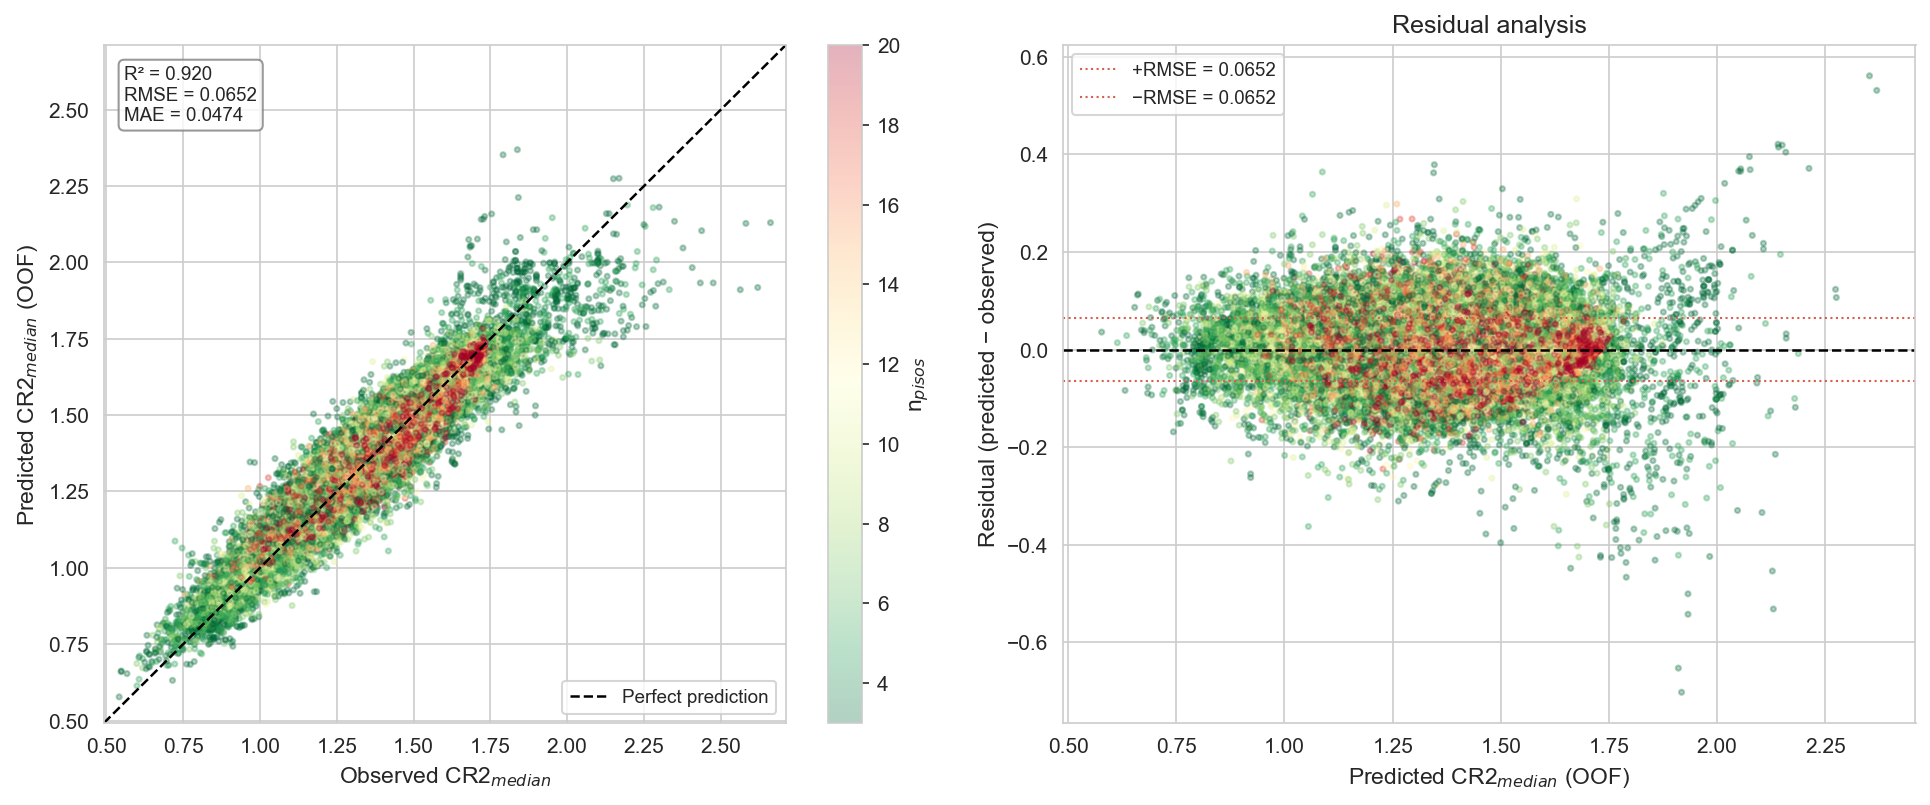
\includegraphics[width=\linewidth]{figs/F2_predicted_vs_actual_oof.png}
\caption{Out-of-fold predicted vs.\ observed $\CR{med}$ (XGBoost). Color
indicates building height $\np$. Dashed line: perfect prediction.
$\Rsq = 0.92$, $\RMSE = 0.065$.}
\label{fig:pred_vs_actual}
\end{figure}

\begin{figure}[htbp]
\centering
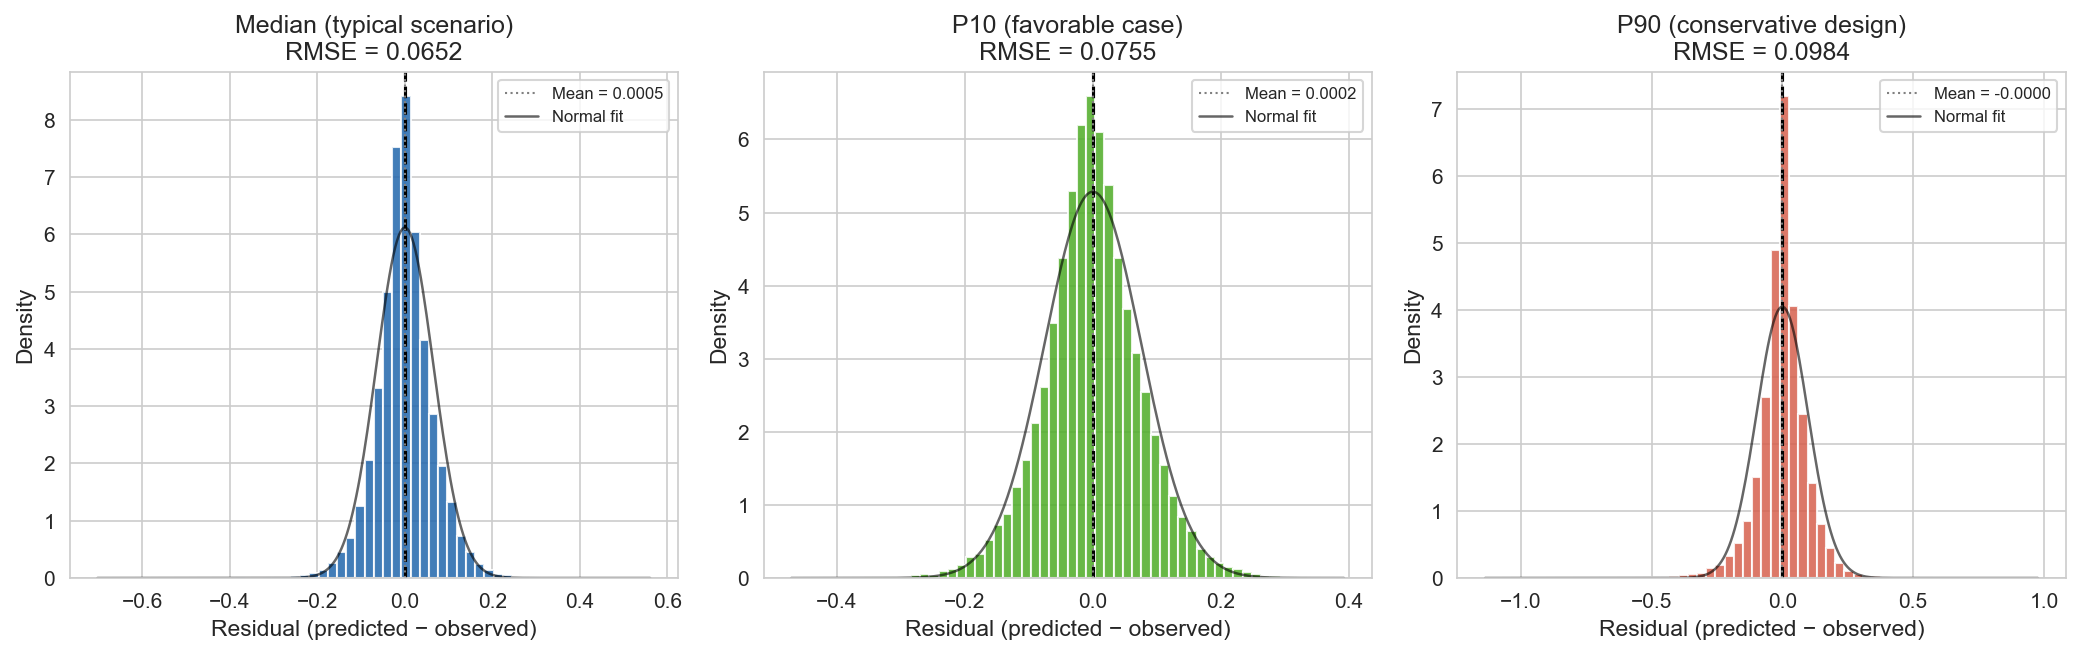
\includegraphics[width=\linewidth]{figs/F3_residual_distributions.png}
\caption{Residual distributions (OOF, XGBoost) for the three $CR_2$ target
variables. Dashed line: zero-mean reference; solid curve: normal fit.}
\label{fig:residuals}
\end{figure}

\begin{figure}[htbp]
\centering
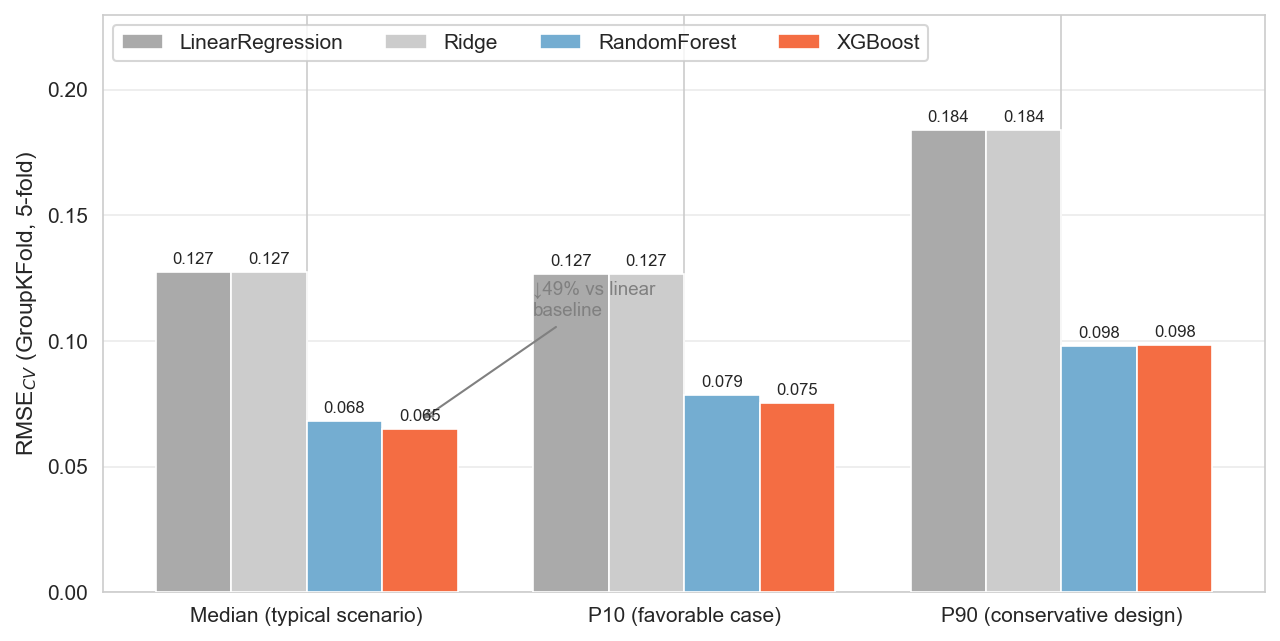
\includegraphics[width=0.85\linewidth]{figs/F1_model_comparison_rmse.png}
\caption{Cross-validated RMSE across models and target variables.
Ensemble methods achieve approximately half the error of linear baselines.}
\label{fig:model_comparison}
\end{figure}

\subsection{Design Variable Hierarchy and Feature Importance}
\label{sec:results:importance}

\Cref{fig:feat_importance} presents the top-12 features for each target,
derived from the XGBoost model. Across all three scenarios, damper density
$\etad$ consistently ranks as the most influential predictor, with a Pearson
correlation $r = -0.73$ with $\CR{med}$. The absolute damper count $\nd$ yields
a substantially weaker correlation ($r = -0.45$), demonstrating that height
normalization is essential: the same $\nd$ represents fundamentally different
levels of structural intervention in a 5-story versus a 20-story frame.

Normalized energy dissipation ($r = -0.70$) ranks second, consistent with the
physical mechanism: greater cumulative dissipation per story reduces peak demand.
The vertical spread of damper positions $\sigma_p$ ($r = -0.54$) ranks third,
indicating that distributed configurations outperform clustered ones. The
friction moment $\Mf$ shows a weaker marginal correlation ($r = -0.19$) but
interacts strongly with $\etad$, as shown in \cref{sec:results:interaction}.

A notable cross-scenario difference is observed in the relative importance of
$\Mf$: its importance rank increases for $\CR{P90}$, suggesting that under
the most demanding records, device-level capacity becomes more relevant than
coverage fraction alone.

\begin{figure}[htbp]
\centering
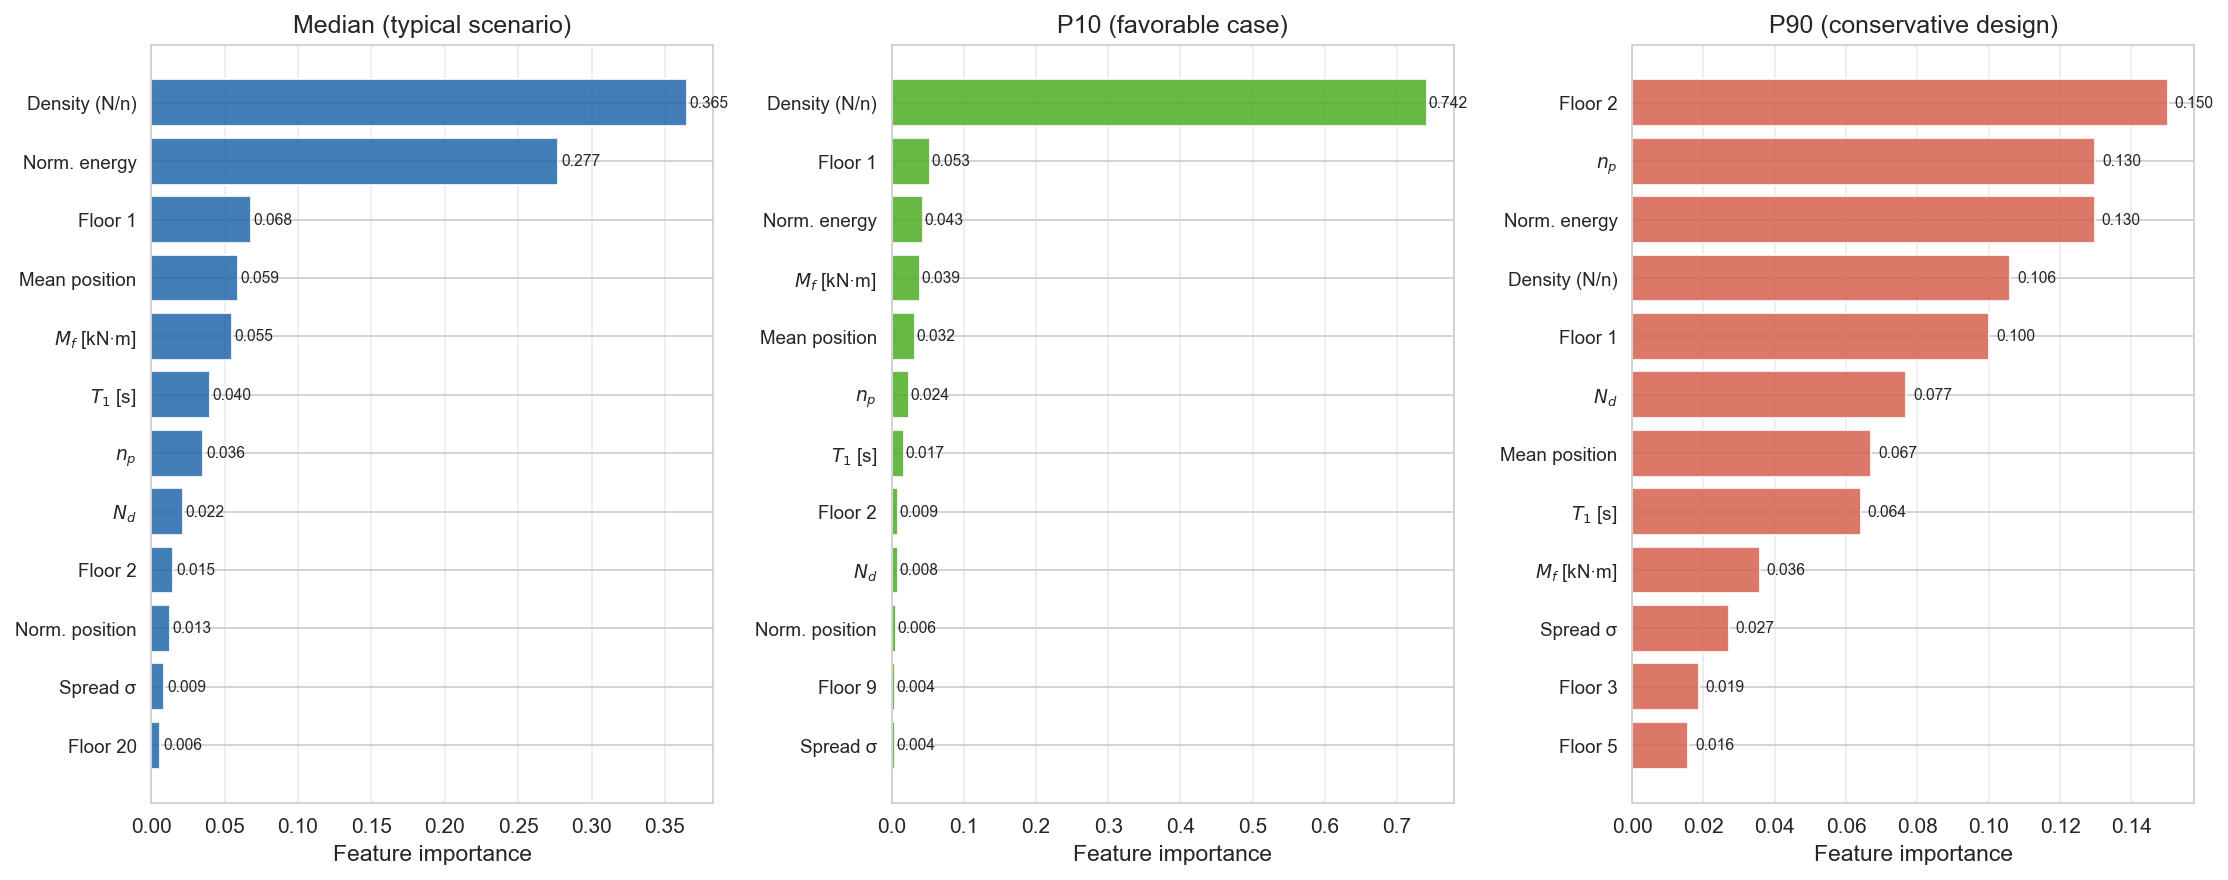
\includegraphics[width=\linewidth]{figs/F4_feature_importance_3targets.png}
\caption{Feature importance (XGBoost) for the top-12 predictors across the
three $CR_2$ target scenarios. Horizontal bars indicate mean impurity
decrease, normalized within each model.}
\label{fig:feat_importance}
\end{figure}

\subsection{Diminishing Returns: Effect of Damper Density on Performance}
\label{sec:results:diminishing}

\Cref{fig:diminishing} investigates the diminishing-returns relationship between
$\etad$ and $CR_2$. For each structure, the best achievable $\CR{med}$ at each
$\nd$ value was identified by selecting the minimum $CR_2$ across all
configurations sharing that count. Performance curves are stratified by building
height to remove the confounding effect of $\np$ on the absolute $\nd$ axis.

The curves confirm a consistent diminishing-returns pattern in all height
categories, with the steepest improvement in the range $\etad \in [0.30,\,0.60]$.
Beyond $\etad = 0.60$, the marginal gain per additional story covered decreases
monotonically. A threshold analysis based on the within-structure normalized
gain (\cref{fig:within_structure}) indicates that 80\,\% of the maximum
achievable performance improvement is captured at $\etad \approx 0.85$ for
mid-rise (6--10 stories), high-rise (11--15 stories), and tall (16--20 stories)
frame categories. Low-rise frames (3--5 stories) require $\etad \approx 0.95$
to reach the same 80\,\% threshold, attributed to the proportionally larger
impact of each additional device in shorter buildings.

\begin{figure}[htbp]
\centering
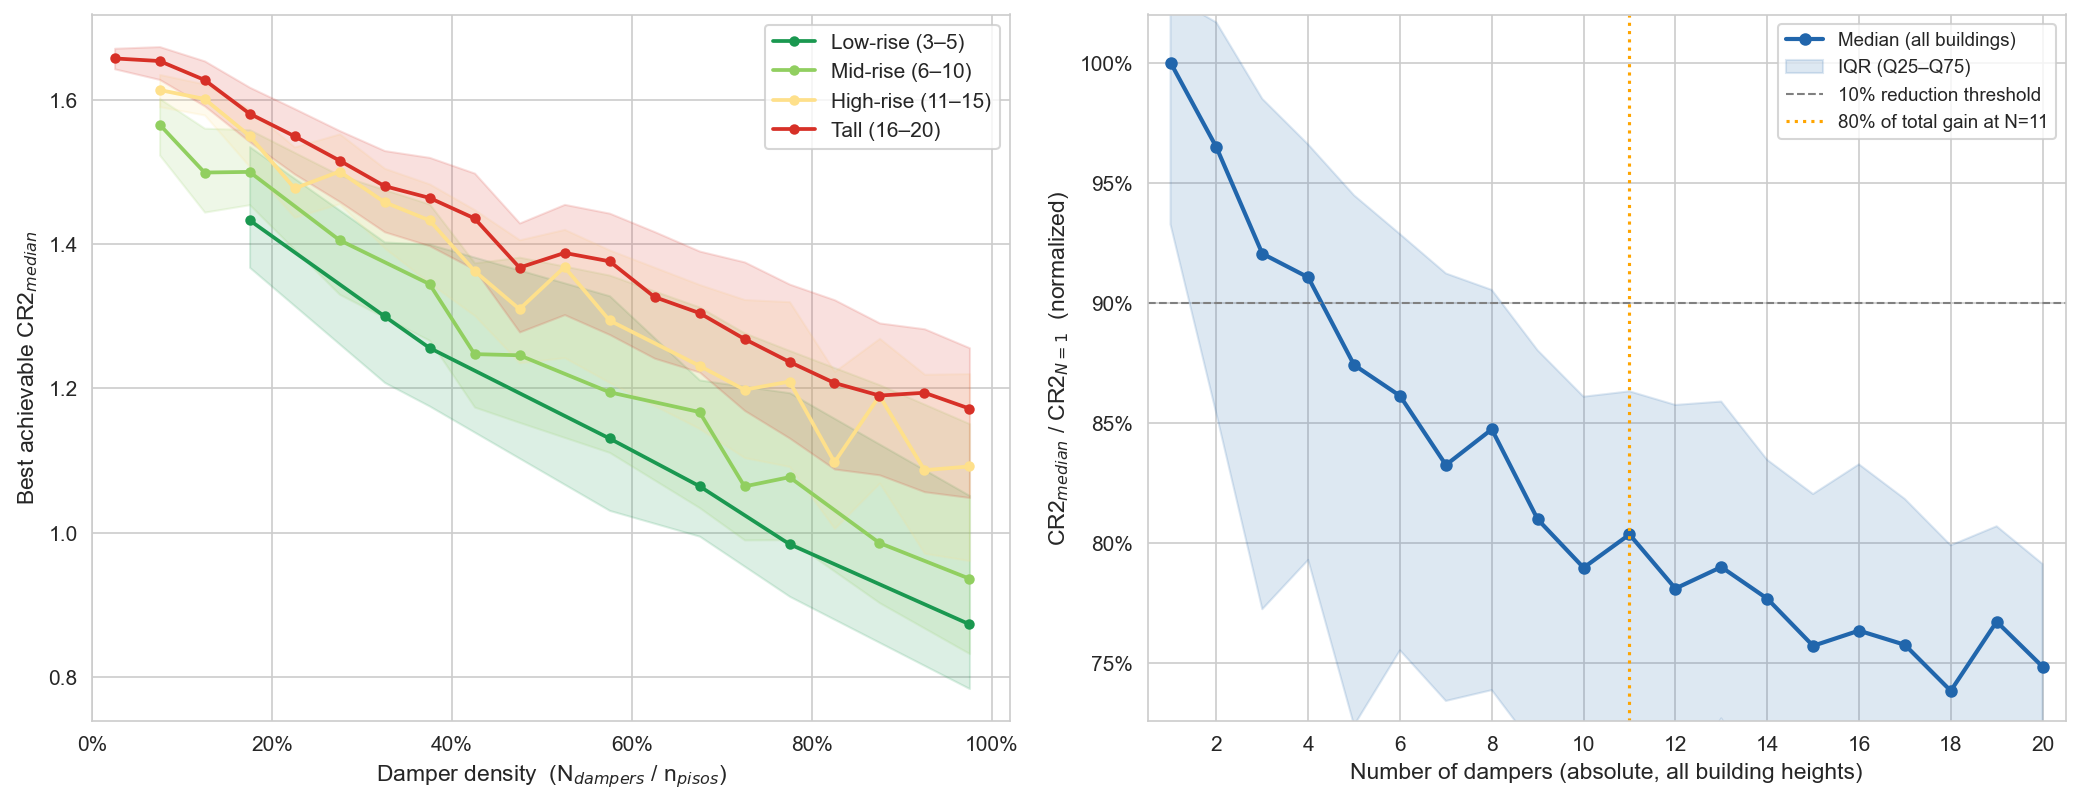
\includegraphics[width=\linewidth]{figs/F5_diminishing_returns.png}
\caption{Left: best achievable $\CR{med}$ vs.\ coverage density $\etad$,
stratified by building height (median $\pm$ IQR). Right: normalized $CR_2$
vs.\ absolute $\nd$ across all buildings (note: confounded with height;
left panel provides the appropriate comparison).}
\label{fig:diminishing}
\end{figure}

\begin{figure}[htbp]
\centering
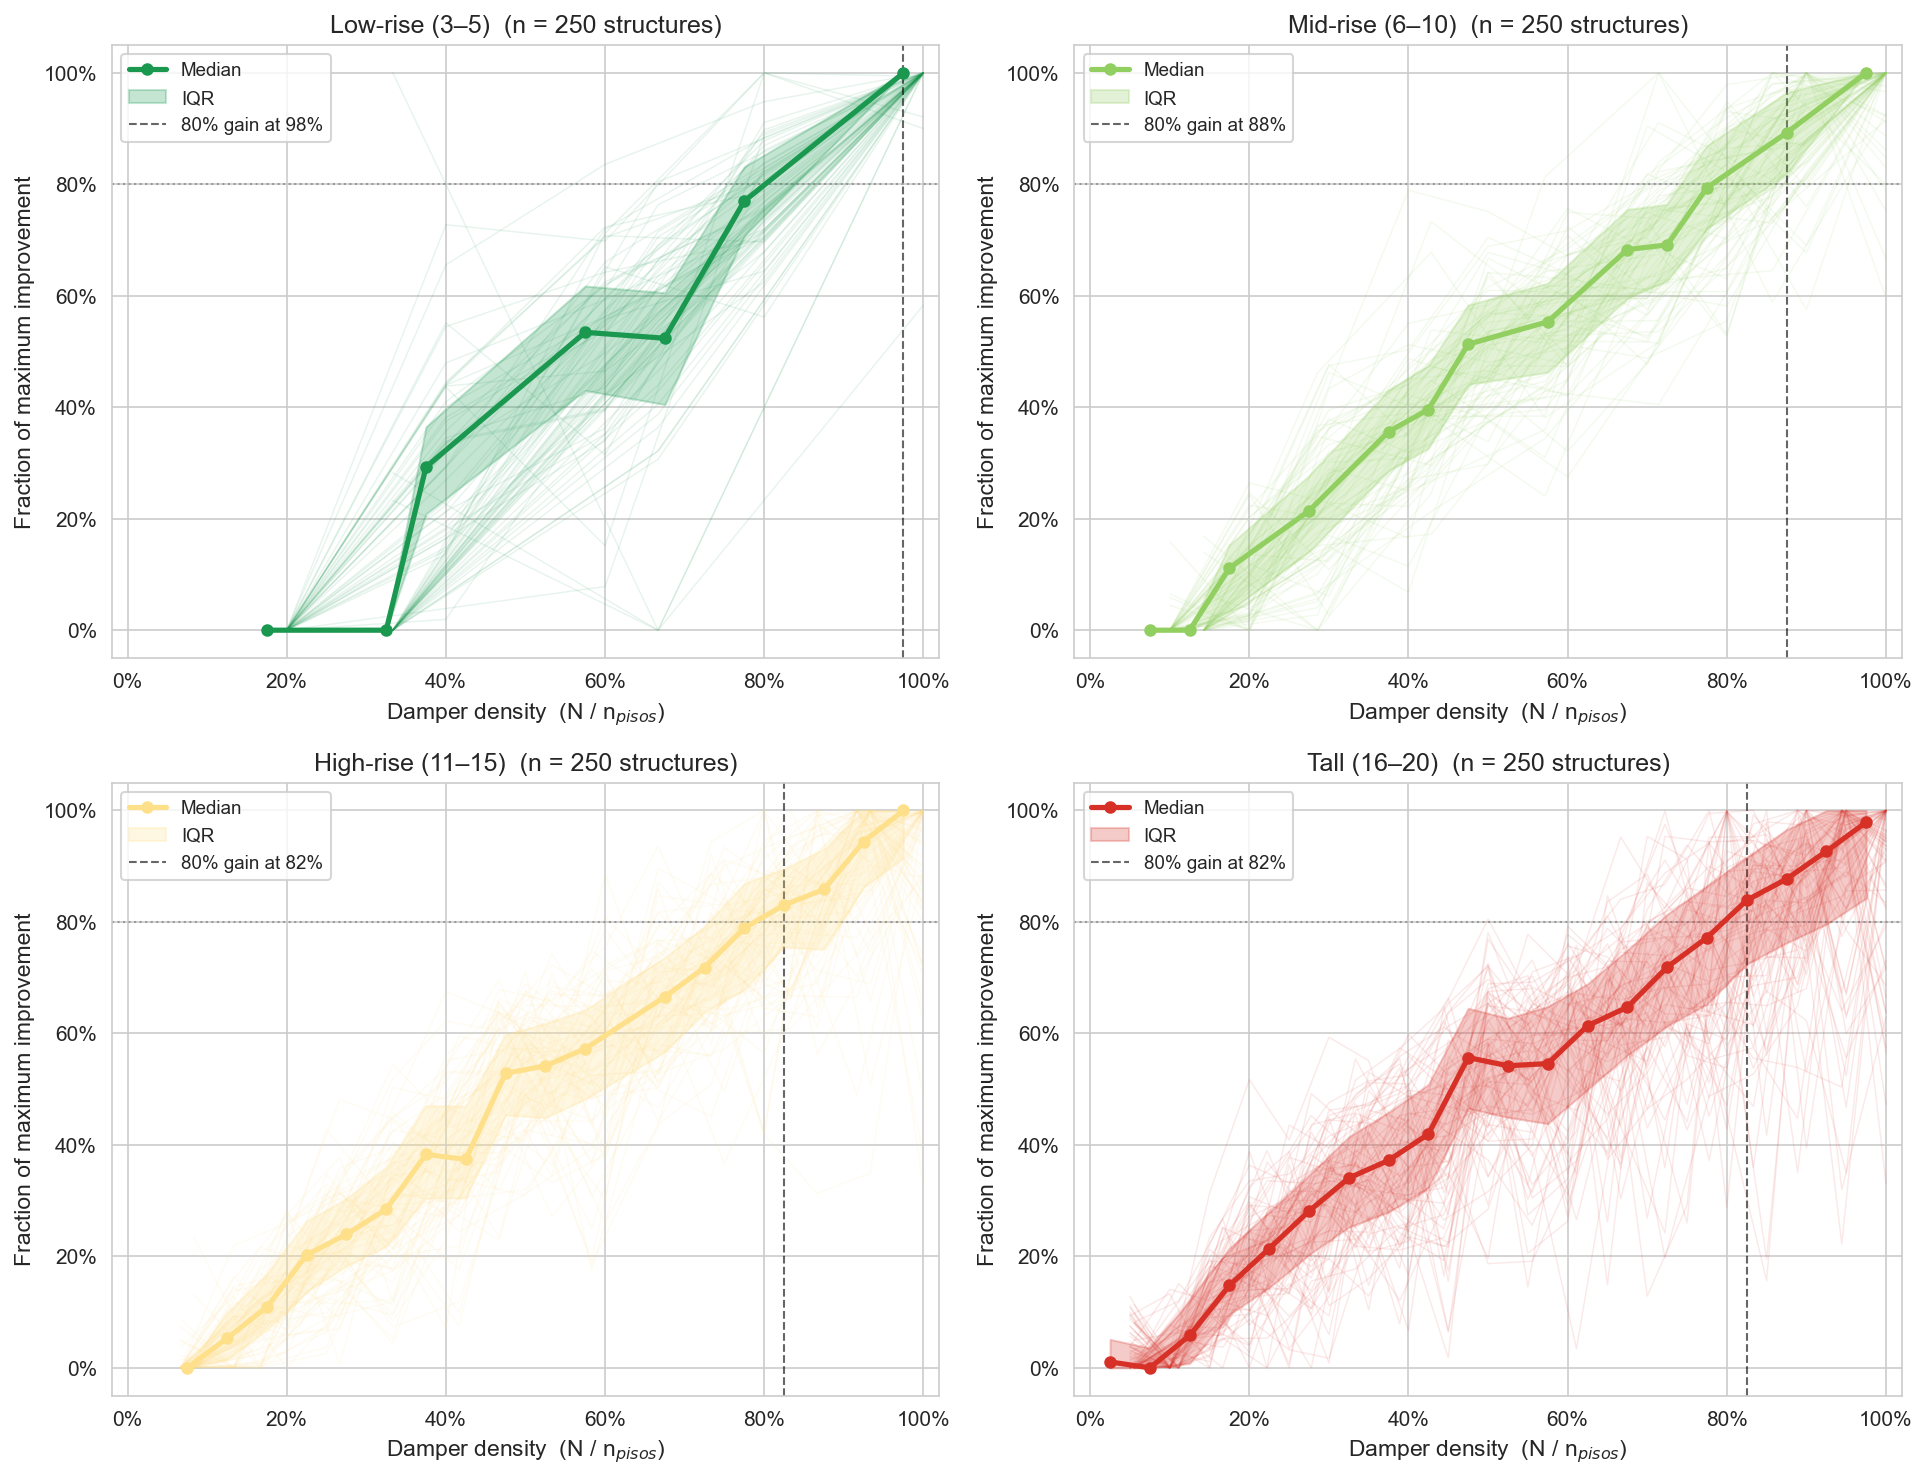
\includegraphics[width=\linewidth]{figs/F6_within_structure_curves.png}
\caption{Within-structure diminishing-returns curves by height group.
Each thin line represents a single structure; thick line is the group median
$\pm$ IQR. Vertical dashed line: density at which 80\,\% of maximum gain
is achieved.}
\label{fig:within_structure}
\end{figure}

\subsection{Interaction Between Damper Quantity and Friction Moment}
\label{sec:results:interaction}

\Cref{fig:heatmap} presents a two-dimensional heat map of the median $CR_2$ as
a function of binned $\nd$ and $\Mf$ across all structures and records.
Three behaviorally distinct regions are identified.

First, low density combined with low $\Mf$ ($\leq$\!100\KM) produces the
highest $CR_2$ values. Second, increasing $\nd$ from 1--2 to 5--6 with
$\Mf \in [200,\,300]$\KM yields $CR_2$ reductions comparable to those achieved
by doubling $\Mf$ at fixed count, indicating a substitution relationship between
quantity and capacity at intermediate levels. Third, for $\nd \geq 9$ the
response becomes relatively insensitive to $\Mf$ within [200,\,500]\KM,
suggesting that at high coverage fractions, placement strategy dominates over
per-device capacity.

The optimal configurations identified across the 1\,000 structures concentrate
in $\Mf \in [300,\,460]$\KM (median 400\KM, IQR [269,\,456]\KM) with coverage
fractions predominantly at or near unity ($\tilde{\eta}_{0.50} = 1.0$).

\begin{figure}[htbp]
\centering
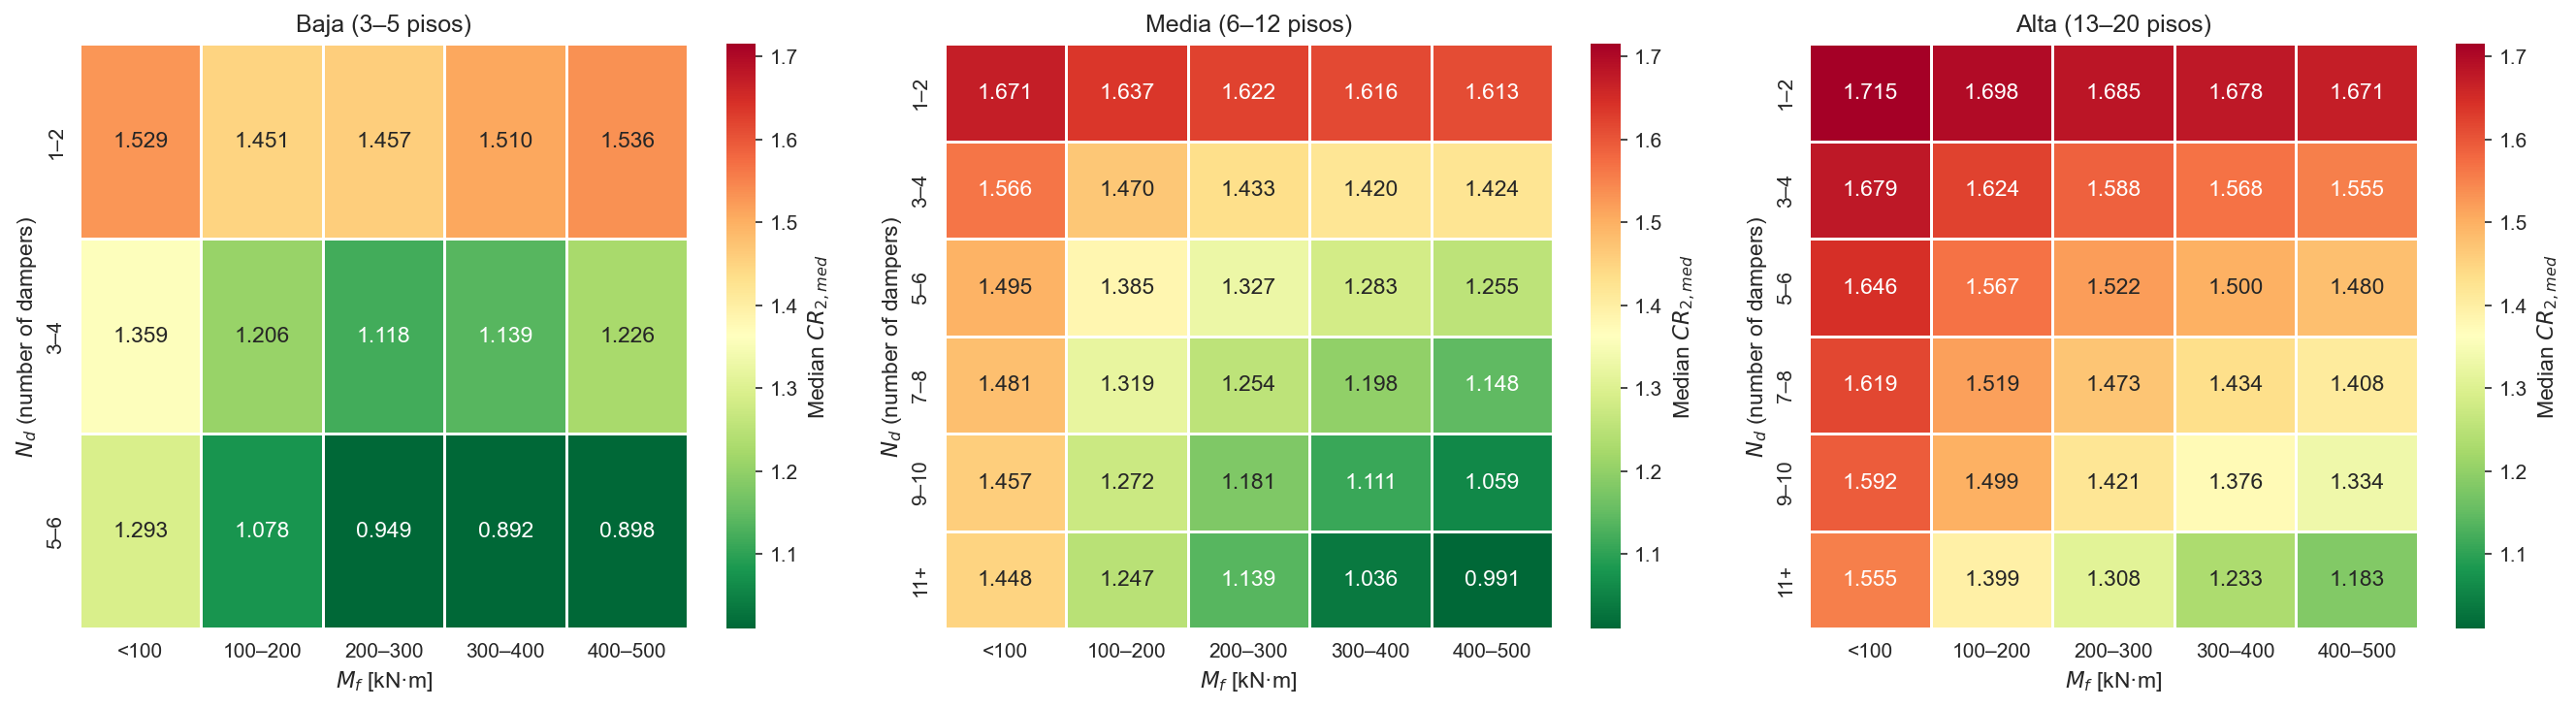
\includegraphics[width=\linewidth]{figs/F7_interaction_heatmap.png}
\caption{Left: median $CR_2$ as a function of $\nd$ bins and $\Mf$ bins
(kN$\cdot$m), averaged over all structures and records. Right: optimal $\nd$
vs.\ $\Mf$ for the best configuration of each structure (color: achieved
$\CR{med}$).}
\label{fig:heatmap}
\end{figure}

\subsection{Design Convergence Across Seismic Scenarios}
\label{sec:results:convergence}

\Cref{fig:convergence} examines whether a single optimal design is robust across
the three seismic scenarios. For each of the 1\,000 structures, the
model-predicted optimal $\nd$ under each target was compared. The distribution
of recommended $\nd$ is broadly consistent: the median and P10 scenarios produce
nearly identical recommendations in most structures. The P90 scenario tends to
recommend slightly higher $\nd$ for taller buildings, but the absolute
discrepancy $|\nd^{\mathrm{P90}} - \nd^{\mathrm{med}}|$ remains below 2 for
more than 80\,\% of structures. This implies that a median-scenario design
provides near-optimal protection across the full range of seismic variability
captured by the eight-record ensemble.

\begin{figure}[htbp]
\centering
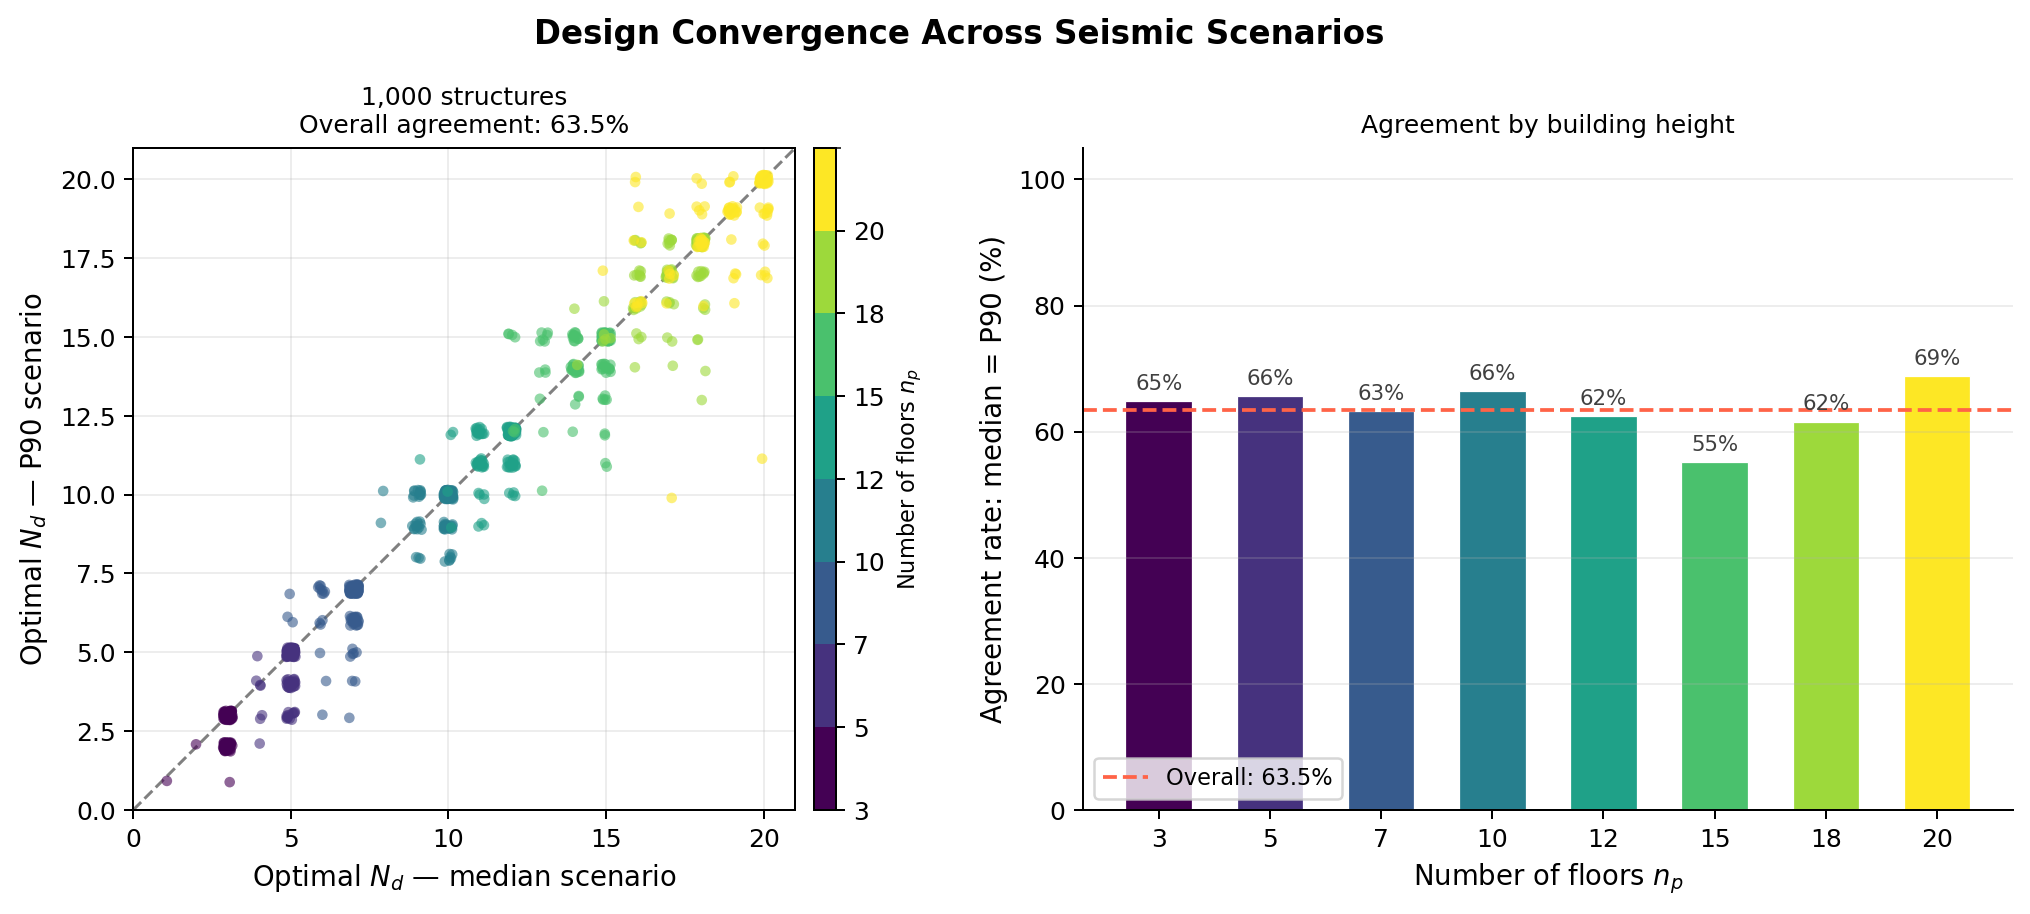
\includegraphics[width=\linewidth]{figs/F8_convergence_extended.png}
\caption{Left: distribution of recommended $\nd$ by seismic scenario across
all 1\,000 structures. Right: agreement rate and mean absolute discrepancy
$|\nd^{\mathrm{P90}} - \nd^{\mathrm{med}}|$ by building height $\np$.}
\label{fig:convergence}
\end{figure}

%%═══════════════════════════════════════════════════════════════════════════
\section{Discussion}
\label{sec:discussion}
%%═══════════════════════════════════════════════════════════════════════════

\subsection{Density as the Governing Design Parameter}

The identification of $\etad = \nd/\np$ as the dominant predictor of $CR_2$
($r = -0.73$) has a direct implication for design practice. Previous
optimization studies, including \citet{Jarrahi2020jbe,Jarrahi2020sdee}, report
results in terms of absolute $\nd$ for a specific reference structure. This
framing limits transferability: the optimal $\nd = 6$ recommended for a
10-story frame by \citet{Jarrahi2020sdee} corresponds to $\etad = 0.60$, while
the same count in a 20-story frame would represent only $\etad = 0.30$ ---
a fundamentally different level of intervention. The present results demonstrate
that once $\nd$ is normalized to $\etad$, performance curves for 6--20 story
structures collapse onto a consistent trend (see \cref{fig:diminishing}, left),
making coverage fraction the appropriate metric for design guidelines.

A preliminary recommendation from the 80\,\% threshold analysis is
$\etad \geq 0.85$ for mid-to-high-rise frames and $\etad \geq 0.90$ for
low-rise frames.

\subsection{Reconciliation with Jarrahi et al.\ (2020): Energy vs.\ Displacement Criteria}

\citet{Jarrahi2020sdee} reported that the energy-based objective
$f = E_i / E_{\mathrm{RFDs}}$ saturates at $\etad \approx 0.60$ for a
10-story SMRF, coinciding with the point at which the cumulative hysteretic
energy $E_h$ of the structural frame drops to approximately zero (no more
structural yielding). The present study, using $CR_2$, finds saturation at
$\etad \approx 0.85$ for the same height category. The difference reflects
metric sensitivity: the energy-based criterion detects the onset of an elastic
structural state as a binary threshold; $CR_2$ continues to differentiate
configurations after yielding has been suppressed, tracking residual
displacement amplification and acceleration demands. The two thresholds are
therefore complementary:
\begin{itemize}
    \item $\etad \geq 0.60$: structural damage prevention (the
          \citealt{Jarrahi2020sdee} criterion, energy-based);
    \item $\etad \geq 0.85$: serviceability control --- peak displacements
          and accelerations cease to respond meaningfully to additional coverage.
\end{itemize}
A design targeting structural protection alone should satisfy the first
criterion; a design additionally controlling serviceability and non-structural
damage should target the second.

\subsection{Interaction Between Friction Moment and Coverage}

The heat map analysis (\cref{fig:heatmap}) reveals a substitution relationship
between $\nd$ and $\Mf$ at intermediate coverage levels: doubling $\Mf$ at
fixed count yields similar $CR_2$ reductions to increasing $\nd$ by two stories.
This interaction is not captured by marginal correlation analysis and motivates
the use of ensemble ML models that represent nonlinear feature interactions
explicitly. At high coverage ($\etad \geq 0.75$), performance becomes relatively
insensitive to the specific $\Mf$ level within [200,\,500]\KM, and the
ML-identified optimal range $\Mf \in [300,\,460]$\KM is consistent with the
optimal $\Mf = 257.9$\,kips$\cdot$in $\approx 290$\KM reported by
\citet{Jarrahi2020jbe} for a single-story SMRF under a higher-intensity input.

\subsection{Scenario Robustness}

The high agreement between median and P90 design recommendations
(\cref{fig:convergence}) implies that it is unnecessary to solve separate
optimization problems for different seismic hazard levels when the goal is to
identify the optimal $\nd$. The multi-record approach directly addresses the
limitation of single-record optimization studies \citep{Jarrahi2020jbe,
Jarrahi2020sdee} by capturing record-to-record variability in the P10, median,
and P90 statistics, making the ML recommendations inherently robust to ground
motion selection uncertainty.

\subsection{Limitations}

The following limitations should be noted. (i)~Structural models are idealized
elastic shear frames; inelastic frame-RFD interaction is not explicitly captured.
(ii)~The eight accelerograms, while seismically diverse, may not represent all
relevant tectonic environments. (iii)~Model validation is based solely on
cross-validation; an independent held-out test set would provide a more
stringent generalization assessment. (iv)~A uniform $\Mf$ per structure is
assumed; story-specific distributions may be preferable in practice. (v)~No
cost function is incorporated, so the economic optimization of coverage fraction
is not addressed.

%%═══════════════════════════════════════════════════════════════════════════
\section{Conclusions}
\label{sec:conclusions}
%%═══════════════════════════════════════════════════════════════════════════

The following principal conclusions are drawn from the analysis of
$\approx$434\,000 nonlinear time-history simulations across 1\,000 structurally
diverse configurations and eight real seismic records:

\begin{enumerate}

\item \textbf{ML surrogate accuracy.} XGBoost and Random Forest achieved
cross-validated $\Rsq$ of 0.92--0.93 for $\CR{med}$ and $\CR{P10}$, and 0.84
for $\CR{P90}$. Ensemble models reduced prediction error by $\approx$49\,\%
relative to linear baselines, quantifying the nonlinear structure of the
design-performance relationship.

\item \textbf{Damper density is the primary design variable.}
The coverage fraction $\etad = \nd/\np$ is the single most influential
predictor ($r = -0.73$), substantially exceeding the correlation of the
absolute count ($r = -0.45$). Design guidelines for RFDs should be expressed
in terms of $\etad$, not $\nd$.

\item \textbf{Diminishing-returns threshold: $\etad \approx 0.85$.}
Within-structure analysis reveals that 80\,\% of the maximum achievable $CR_2$
reduction is captured at $\etad \approx 0.85$ for mid-to-high-rise frames
(6--20 stories) and $\etad \approx 0.95$ for low-rise frames (3--5 stories).
These thresholds provide practical cost-effectiveness criteria for RFD deployment.

\item \textbf{Reconciliation with the energy-based threshold of Jarrahi et al.}
\citet{Jarrahi2020sdee} reported saturation of the energy-based objective at
$\etad \approx 0.60$ (structural yielding eliminated). The present
displacement-based criterion finds saturation at $\etad \approx 0.85$, 25
percentage points higher. The difference is explained by the greater sensitivity
of $CR_2$ to displacement and acceleration demands that persist beyond the
structural yield threshold. The two criteria describe complementary performance
levels: $\etad \geq 0.60$ targets damage prevention; $\etad \geq 0.85$
additionally targets serviceability.

\item \textbf{Optimal friction moment range.} Across all 1\,000 structures,
the ML-identified optimal $\Mf$ concentrates in [300,\,460]\KM (median
400\KM). At $\etad \geq 0.75$, $CR_2$ is relatively insensitive to $\Mf$
within [200,\,500]\KM, so coverage fraction is the more critical design lever.

\item \textbf{Scenario robustness.} The optimal $\nd$ recommended by the
median and P90 scenarios differs by fewer than 2 stories in 80\,\% of analyzed
structures, confirming that a single median-optimized design provides near-optimal
protection across the range of seismic variability captured by the eight-record
ensemble.

\item \textbf{Future work.} Extensions should incorporate inelastic frame
behavior, story-specific $\Mf$ distributions, installation cost constraints, and
broader seismic record suites. Experimental validation for multi-story
configurations and integration into an interactive design tool represent immediate
research directions.

\end{enumerate}

%%═══════════════════════════════════════════════════════════════════════════
%% Bibliography
%%═══════════════════════════════════════════════════════════════════════════
\bibliographystyle{elsarticle-harv}   % APA-style author-year
\bibliography{references}

\end{document}
